\begin{tikzpicture}[font=\small]
  % left: x^2 + 7x + 6
  \begin{scope}
    \draw[thick] (-0.8,-0.8) -- (0.8,0.8);
    \draw[thick] (-0.8,0.8) -- (0.8,-0.8);
    \node at (0,0.75) {$7$};
    \node at (0,-0.75) {$6$};
    \node at (-0.75,0) {$6$};
    \node at (0.75,0) {$1$};
    \node[align=center] at (0,-1.6) {$x^2+7x+6$\\ top: $b=7$, bottom: $ac=6$};
  \end{scope}
  % right: 3x^2 + 5x + 2
  \begin{scope}[xshift=5cm]
    \draw[thick] (-0.8,-0.8) -- (0.8,0.8);
    \draw[thick] (-0.8,0.8) -- (0.8,-0.8);
    \node at (0,0.75) {$5$};
    \node at (0,-0.75) {$6$};
    \node at (-0.85,0) {$\dfrac{3}{3}$};
    \node at (0.85,0) {$\dfrac{2}{3}$};
    \node[blue] at (-1.9,0) {$(x+1)$};
    \node[blue] at (2.05,0) {$(3x+2)$};
    \node[align=center] at (0,-1.6) {$3x^2+5x+2$\\ sides divided by $a=3$};
  \end{scope}
\end{tikzpicture}
